\documentclass{beamer}
\usetheme{Szeged}
\usecolortheme{beaver}

\usepackage{tikz}
\usetikzlibrary{positioning}
\tikzset{
    auto,
    circle,
    draw,
    node distance = 0.6cm,
    minimum size = 0.8cm,
    r/.style = {draw = red, line width = 0.05cm, fill=red!50},
    b/.style = {draw = black, line width = 0.05cm, fill=black!20},
    a/.style = {draw = black, line width = 0.01cm, fill=black!3},
    i/.style = {dashed}
}

\usepackage{minted}
\usemintedstyle{pastie}
\newcommand{\code}[1]{\mintinline{ocaml}{#1}}

\title{Discussion 12}
\subtitle{Balanced Trees}
\author{Kenneth Fang (kwf37), Newton Ni (cn279)}

\begin{document}

    \begin{frame}
        \titlepage{}
    \end{frame}
    
    \begin{frame}{Key Ideas}
        \begin{itemize}
            \item<1-> Red-Black Trees
            \begin{itemize}
                \item<2-> Invariants
                \item<3-> Insertion
                \item<4-> Deletion
            \end{itemize}
        \end{itemize}
    \end{frame}

    \begin{frame}[fragile=singleslide]{Type}
        \begin{minted}[autogobble]{ocaml}
            type color =
            | R
            | B

            type 'a tree =
            | Leaf
            | Node of color * 'a * 'a tree * 'a tree
        \end{minted} 
    \end{frame}

    \begin{frame}{Invariants}
        \begin{itemize}
            \item Convention: root node is black
        \end{itemize} 
    \end{frame}

    \begin{frame}
        \begin{figure}
        \begin{tikzpicture}
            \begin{scope}
                \node[r] (1) at (0, 0) [label=above:BAD];
                \node[b] (2) [below left = of 1]        ; 
                \node[b] (3) [below right = of 1]       ; 

                \path (1) edge (2) --
                      (1) edge (3);
            \end{scope}

            \pause

            \begin{scope}
                \node[b] (1) at (6, 0) [label=above:GOOD];
                \node[r] (2) [below left = of 1]         ; 
                \node[r] (3) [below right = of 1]        ; 

                \path (1) edge (2) --
                      (1) edge (3);
            \end{scope}

        \end{tikzpicture}
        \end{figure}
    \end{frame}

    \begin{frame}{Invariants}
        \begin{itemize}
            \item There are no two adjacent red nodes along any path
        \end{itemize} 
    \end{frame}

    \begin{frame}
        \begin{figure}
        \begin{tikzpicture}
            \begin{scope}
                \node[b] (1) at (0, 0) [label=above:BAD];
                \node[r] (2) [below left = of 1]        ;
                \node[b] (3) [below right = of 1]       ;
                \node[r] (4) [below left = of 2]        ;

                \path (1) edge (2) --
                      (1) edge (3) --
                      (2) edge (4);
            \end{scope}

            \pause

            \begin{scope}
                \node[b] (1) at (6, 0) [label=above:GOOD];
                \node[r] (2) [below left = of 1]         ;
                \node[b] (3) [below right = of 1]        ;
                \node[b] (4) [below left = of 2]         ;

                \path (1) edge (2) --
                      (1) edge (3) --
                      (2) edge (4);
            \end{scope}
        \end{tikzpicture}
        \end{figure}
    \end{frame}

    \begin{frame}{Invariants}
        \begin{itemize}
            \item Every path from root to leaf has equal number of \textbf{black} nodes
        \end{itemize} 
    \end{frame}

    \begin{frame}
        \begin{figure}
        \begin{tikzpicture}
            \begin{scope}
                \node[b] (1) at (0, 0) [label=above:BAD];
                \node[r] (2) [below left = of 1]        ;
                \node[b] (3) [below right = of 1]       ;

                \path (1) edge (2) --
                      (1) edge (3);
            \end{scope}

            \pause

            \begin{scope}
                \node[b] (1) at (6, 0) [label=above:GOOD];
                \node[b] (2) [below left = of 1]         ;
                \node[b] (3) [below right = of 1]        ;

                \path (1) edge (2) --
                      (1) edge (3);
            \end{scope}
        \end{tikzpicture}
        \end{figure}
    \end{frame}

    \begin{frame}{Insertion}
        \begin{itemize}
            \item<1-> Assume invariants hold before insertion
            \item<2-> Fix invariants after insertion
        \end{itemize} 
    \end{frame}

    \begin{frame}{Insertion: Easy Cases}
        \begin{figure}
        \begin{tikzpicture}
            \begin{scope}
                \node[b]    (1) at (0, 0) [label=above:1];
                \node[r, i] (2) [below left = of 1]      ;

                \path (1) edge (2);
            \end{scope}

            \pause

            \begin{scope}
                \node[b]    (1) at (5, 0) [label=above:2];
                \node[r, i] (2) [below right = of 1]     ;

                \path (1) edge (2);
            \end{scope}

            \pause

            \begin{scope}
                \node[b]    (1) at (0, -3) [label=above:3];
                \node[r, i] (2) [below left = of 1]       ;
                \node[r]    (3) [below right = of 1]      ;

                \path (1) edge (2) --
                      (1) edge (3);
            \end{scope}

            \pause

            \begin{scope}
                \node[b]    (1) at (5, -3) [label=above:4];
                \node[r]    (2) [below left = of 1]       ;
                \node[r, i] (3) [below right = of 1]      ;

                \path (1) edge (2) --
                      (1) edge (3);
            \end{scope}

        \end{tikzpicture}
        \end{figure}
    \end{frame}

    \begin{frame}{Insertion: Hard Cases}
        \begin{figure}
        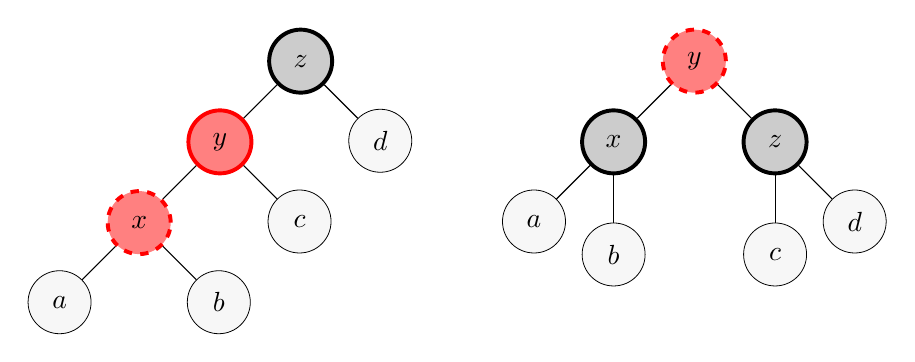
\begin{tikzpicture}
            \begin{scope}
                \node[b]    (1) at (0, 0)            {$z$};
                \node[r]    (2) [below left = of 1]  {$y$};
                \node[a]    (3) [below right = of 1] {$d$};
                \node[r, i] (4) [below left = of 2]  {$x$};
                \node[a]    (5) [below left = of 4]  {$a$};
                \node[a]    (6) [below right = of 4] {$b$};
                \node[a]    (7) [below right = of 2] {$c$};

                \path (1) edge (2) --
                      (1) edge (3) --
                      (2) edge (4) --
                      (2) edge (7) --
                      (4) edge (5) --
                      (4) edge (6);
            \end{scope}

            \pause

            \begin{scope}
                \node[r, i] (1) at (5, 0)            {$y$};
                \node[b]    (2) [below left = of 1]  {$x$};
                \node[b]    (3) [below right = of 1] {$z$};
                \node[a]    (4) [below left = of 2]  {$a$};
                \node[a]    (5) [below = of 2] {$b$};
                \node[a]    (6) [below = of 3]  {$c$};
                \node[a]    (7) [below right = of 3] {$d$};

                \path (1) edge (2) --
                      (1) edge (3) --
                      (2) edge (4) --
                      (2) edge (5) --
                      (3) edge (6) --
                      (3) edge (7);
            \end{scope}
        \end{tikzpicture}
        \end{figure}
    \end{frame}

    \begin{frame}{Insertion: Hard Cases}
        \begin{figure}
        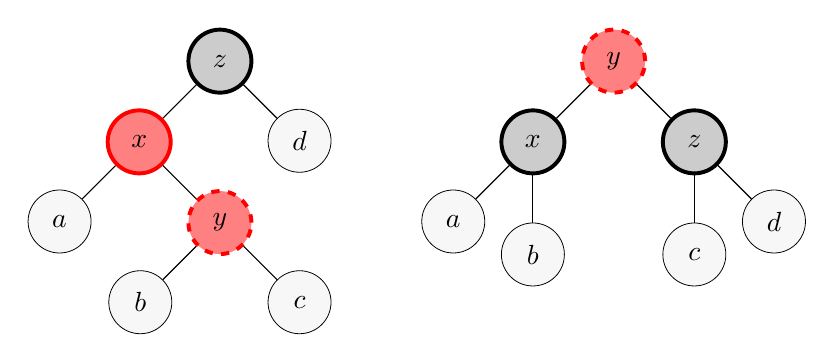
\begin{tikzpicture}
            \begin{scope}
                \node[b]    (1) at (0, 0)            {$z$};
                \node[r]    (2) [below left = of 1]  {$x$};
                \node[a]    (3) [below right = of 1] {$d$};
                \node[r, i] (4) [below right = of 2] {$y$};
                \node[a]    (5) [below left = of 4]  {$b$};
                \node[a]    (6) [below right = of 4] {$c$};
                \node[a]    (7) [below left = of 2]  {$a$};

                \path (1) edge (2) --
                      (1) edge (3) --
                      (2) edge (4) --
                      (2) edge (7) --
                      (4) edge (5) --
                      (4) edge (6);
            \end{scope}

            \pause

            \begin{scope}
                \node[r, i] (1) at (5, 0)            {$y$};
                \node[b]    (2) [below left = of 1]  {$x$};
                \node[b]    (3) [below right = of 1] {$z$};
                \node[a]    (4) [below left = of 2]  {$a$};
                \node[a]    (5) [below = of 2] {$b$};
                \node[a]    (6) [below = of 3]  {$c$};
                \node[a]    (7) [below right = of 3] {$d$};

                \path (1) edge (2) --
                      (1) edge (3) --
                      (2) edge (4) --
                      (2) edge (5) --
                      (3) edge (6) --
                      (3) edge (7);
            \end{scope}
        \end{tikzpicture}
        \end{figure}
    \end{frame}
 
    \begin{frame}{Insertion: Hard Cases}
        \begin{figure}
        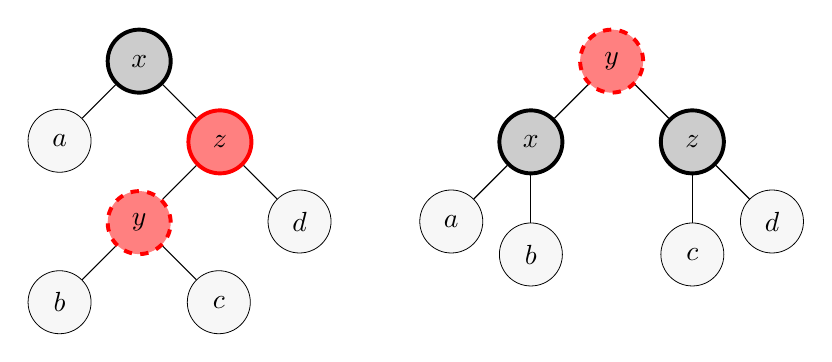
\begin{tikzpicture}
            \begin{scope}
                \node[b]    (1) at (0, 0)            {$x$};
                \node[a]    (2) [below left = of 1]  {$a$};
                \node[r]    (3) [below right = of 1] {$z$};
                \node[r, i] (4) [below left = of 3]  {$y$};
                \node[a]    (5) [below right = of 3] {$d$};
                \node[a]    (6) [below left = of 4]  {$b$};
                \node[a]    (7) [below right = of 4] {$c$};

                \path (1) edge (2) --
                      (1) edge (3) --
                      (3) edge (4) --
                      (3) edge (5) --
                      (4) edge (6) --
                      (4) edge (7);
            \end{scope}

            \pause

            \begin{scope}
                \node[r, i] (1) at (6, 0)            {$y$};
                \node[b]    (2) [below left = of 1]  {$x$};
                \node[b]    (3) [below right = of 1] {$z$};
                \node[a]    (4) [below left = of 2]  {$a$};
                \node[a]    (5) [below = of 2] {$b$};
                \node[a]    (6) [below = of 3]  {$c$};
                \node[a]    (7) [below right = of 3] {$d$};

                \path (1) edge (2) --
                      (1) edge (3) --
                      (2) edge (4) --
                      (2) edge (5) --
                      (3) edge (6) --
                      (3) edge (7);
            \end{scope}
        \end{tikzpicture}
        \end{figure}
    \end{frame}

    \begin{frame}{Insertion: Hard Cases}
        \begin{figure}
        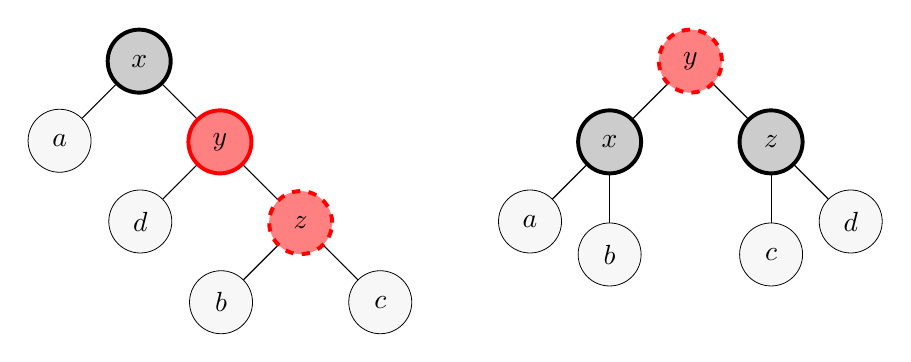
\begin{tikzpicture}
            \begin{scope}
                \node[b]    (1) at (0, 0)            {$x$};
                \node[a]    (2) [below left = of 1]  {$a$};
                \node[r]    (3) [below right = of 1] {$y$};
                \node[r, i] (4) [below right = of 3] {$z$};
                \node[a]    (5) [below left = of 3]  {$d$};
                \node[a]    (6) [below left = of 4]  {$b$};
                \node[a]    (7) [below right = of 4] {$c$};

                \path (1) edge (2) --
                      (1) edge (3) --
                      (3) edge (4) --
                      (3) edge (5) --
                      (4) edge (6) --
                      (4) edge (7);
            \end{scope}

            \pause

            \begin{scope}
                \node[r, i] (1) at (7, 0)            {$y$};
                \node[b]    (2) [below left = of 1]  {$x$};
                \node[b]    (3) [below right = of 1] {$z$};
                \node[a]    (4) [below left = of 2]  {$a$};
                \node[a]    (5) [below = of 2] {$b$};
                \node[a]    (6) [below = of 3]  {$c$};
                \node[a]    (7) [below right = of 3] {$d$};

                \path (1) edge (2) --
                      (1) edge (3) --
                      (2) edge (4) --
                      (2) edge (5) --
                      (3) edge (6) --
                      (3) edge (7);
            \end{scope}
        \end{tikzpicture}
        \end{figure}
    \end{frame}

    \begin{frame}{Insertion: Summary}
        \begin{itemize}
            \item<1-> Similar to regular binary tree insertion
            \item<2-> Reconstruct balanced tree as we insert
            \item<3-> \code{insert l v |> balance |> rep_ok}
        \end{itemize}
    \end{frame}

    \begin{frame}{Deletion}
        \begin{itemize}
            \item<1-> See paper by Germane, Might
            \item<2-> Central idea: introduce \textbf{double-black} node during deletion
            \item<3-> \code{type color = R | B | BB}
        \end{itemize}
    \end{frame}

\end{document}
